\documentclass[
%*********************************************
%* Paper type (letterpaper)                  *
%*********************************************
    a4paper,
%   letterpaper,
%   a5paper,
%   b5paper,
%   executivepaper,
%   legalpaper,
%
%*********************************************
%* Font size (10pt)                          *
%*********************************************
%   10pt,
    11pt,
%   12pt,
%
%*********************************************
%* Paging (document dependent)               *
%*********************************************
    oneside,
%   twoside,
%
%*********************************************
%* Equation alignment (center)               *
%*********************************************
%   fleqn,                  %placerer fomlerne i venstre siden istedet for centreret.
%   leqno,                  %Placerer formelnummereringen på venstre side (istedet for højre)
%
%*********************************************
%* Chapter positioning (document dependent)  *
%*********************************************
    openany,                %openany starter chapters på næstkommende side.
%   openright,
%
%*********************************************
%* Language (none)                           *
%*********************************************
%    english]
   danish]
%
%*********************************************
%* Document type (none)                      *
%*********************************************
%   {book}
    {article}
%   {slides}
%   {report}


%*********************************************
%* Userpackages                              *
%*********************************************
\usepackage[danish]{babel}
%\usepackage{t1enc}          %Bruges til sprog oa.
\usepackage[latin1]{inputenc}
\usepackage{amsfonts}
\usepackage{mathrsfs}
%\usepackage[xdvi]{epsfig}
%\usepackage{ifthen}
%\usepackage{latexsym}
%\usepackage{theorem}
\usepackage[dvips]{graphicx}       %Used when including .eps (graphics) files
%\usepackage{varioref}
%\usepackage{epic}
%\usepackage{eepic}
%\usepackage{rotfloat}
%\usepackage{multicol}
%\usepackage{wrapfig}
%\usepackage{syntonly}          %Use this to check for proper syntax, makes output file.
%\syntaxonly                %Use this to check for proper syntax, makes NO output file.
\usepackage{verbatim}          %Used when to include an unformatted ASCII file
%\usepackage{fancyhdr}
%\usepackage{layout}
%\usepackage{float}
%\usepackage{makeidx}          %Used when making an index in the document
\usepackage{calc}              %Used if you wanna use cm, mm, ex etc. instead of pt

%%
%% For code syntax highliting
%%
%\usepackage{color}
%\usepackage{alltt}

\pagestyle
%*********************************************
%* Header / footer configuration (none)      *
%*********************************************
    {plain}                 %Writes page number in footer, header is empty.
%   {headings}
%   {empty}                 %Makes no header or footer
%   {myheadings}
%   {fancy}



%*********************************************
%* Extra pagelayout    (se s. 110)           *
%*********************************************
%\hoffset   =   -0.5cm %Venstremargin
%\voffset   =   0pt
%\evensidemargin=   0pt
%\oddsidemargin =   0pt %Ekstra venstremargin til dobbeltsider
%\topmargin =   -2cm
%\headheight    =   0pt
%\headsep   =   0pt
%\textheight = 690pt
%\textwidth =   480pt
%\marginparsep  =   0pt
%\marginparwidth=   0pt
%\footskip  =   0pt
%\marginparpush =   0pt
%\paperwidth    =   597pt
%\paperheight   =   845pt

%\makeindex

%\parskip   =   1ex
%\parindent =   0em
%\baselineskip  =   2ex

%\underlineheadings

\title{MPEG �velse}
%
\author{Mikkel Gravgaard - 20043246\\Bent Bisballe Nyeng - 20001467}

\markboth{}{}
%*********************************************
%*                start of                   *
%*              -=DOCUMENT=-                 *
%*********************************************
\begin{document}
\maketitle
\tableofcontents 
% -*- coding: utf-8 -*-
\section{Introduktion}
Vi ønsker i denne øvelse at implementere en lyd-encoder lignende den som benyttes i MPEG 1 Audio layer 1. Nærmere bestemt ønsker vi at implementere subband-kodning og efterfølgende kvantisering baseret på den menneskelige høretærskel samt spektral maskering.

I figur \ref{blokdiagram} vises et blokdiagram over vores encoders konstruktion.

\begin{figure}[h!]
\begin{center}
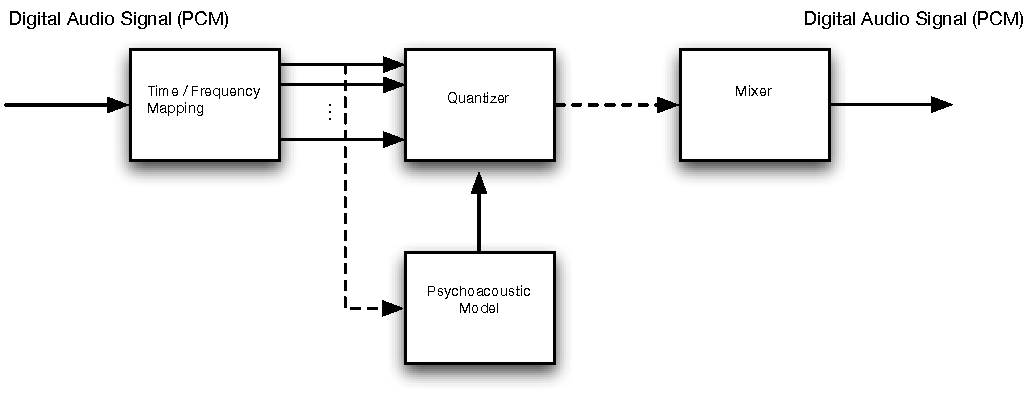
\includegraphics[width=12cm]{blokdiagram}\\
\end{center}
\label{blokdiagram}
\caption{Encoderens konstruktion}
\end{figure}

Der tages ikke højde for MPEG audio-filstandarden; vi ønsker kun at afprøve de tekniske byggeklodser i MPEG audio codec.

% -*- coding: utf-8 -*-
\section{Brugervejledning}
Koden kan afvikles direkte på Mac og Linux. Den kan sandsynligvis også
afvikles på andre platforme, men det vil nok kræve lidt tilpadsning af
udviklingsmiljøet.

Programmet styres af en række parametre, som står hardcodede i
\verb|config.cc|. Disse er flg.:
\begin{verbatim}
float config::ath_weight = 1.0;
float config::mask_weight = 1.0;
float config::quality = 1.0;
mask_t config::mask = MASK_MAX;
filter_t config::filter = FILTER_LOG;
unsigned int config::num_threads = 3;
\end{verbatim}
\verb|ath_weight| er en vægtning af ATH kurven. Denne skal have
værdier mellem 0 og 1.\\
\verb|mask_weight| er en vægtning af maskeringen, denne kan ligeledes
have værdier mellem 0 og 1.\\
\verb|quality| parameteren styrer bittildelings algoritmen
(quantizeren). Værdierne kan være mellem 0 og 1, hvor 1 er fuld pcm
kvalitet og 0 er stilhed. Denne parameter kan være lidt svær at tyre,
men kan med lidt snilde kontrollere output bitraten.\\
\verb|mask| og \verb|filter| styrer begge hvilke algortimer der skal
bruges internt. Der findes flg. maskeringsalgortimer: \verb|MASK_MAX|,
\verb|MASK_BIQUAD| og \verb|MASK_AVG|, samt flg. filtrerings
algortimer: \verb|FILTER_LIN| og \verb|FILTER_LOG|.\\
\verb|num_threads| styrer som navnet antyder, hvor mange tråde
programmet skal bruge. Dette kan med fordel sættes til antalles et
tilgængelige cpuer gange to, minus et.

Disse parametre kan frit ændres, hvorefter programmet skal
genkompileres. Dette gøre ganske enkelt med kommandoen \verb|make|.

Udførslen af programmet foretages med følgende kommando linie, med
dertilhørende parametre: \verb|./soundenc inputfil|.\\
Det er vigtigt at inputfilen er i et wavformat (signed/unsigned,
8/16/32 bit, integer/float baseret), samt at filen er i mono.\\
Overholdes dette ikke giver programmet udefinerede resultater.

Programmet spiller automatisk det beregnede resultat når beregningerne
er fuldført, samt lagrer resultatet i filen \verb|output.wav|, som en 32
bit floatingpoint PCM fil.\\
\\
\textbf{Bemærk; output.wav overskrives uden varsel hvis den findes i
  forvejen!}\\
\\
Koden er afhængig af flg. open source libraries for at kunne kompilere:\\
libsndfile - \verb|http://www.mega-nerd.com/libsndfile|\\
libfftw3 - \verb|http://www.fftw.org|\\
libao - \verb|http://www.xiph.org/ao|

% -*- coding: utf-8 -*-
\section{Båndopsplitning}
\label{sec.subband}
Vi ved hjælp af Matlabs \texttt{fir1}-funktion genereret en båndpas-filterbank med 32 stks 512 pols FIR-filtre. I vores encoder splitter vi kildelyden op i 32 bånd ved at fourier-transformere lyd og filtre og efterfølgende gange disse sammen (svarer til foldning i tidsdomænet). Matlab-programmet til generering af filtrene kan findes i filen \texttt{make\-filters.m}.

Herefter kan hvert af de resulterende 32 bånd iflg. teorien om undersampling nedsamples 32 gange, men dette har vi ikke kunnet få til at fungere uden betydeligt informationstab, så vi skipper derfor undersamplingen i vores encoding, hvilket naturligvis har den konsekvens at den resulterende datamængde bliver 32 gange større.

\section{dfgjsdfgjsdfg}

ath
masking in general
maxmask, avgmask
noget om mask weight

% -*- coding: utf-8 -*-
\subsection*{Biquad-maskering}
De tidligere beskrevne maskeringsmetoder benytter sig kun af
informationer fra de to omkringliggende bånd. Biquad maskering er et
forsøg på at lave alle bånd kunne maskere hinanden, uden at de ved et
uheld kommer til at maskere sig selv.\\
Maskeringskurven er frembragt på gølgende vis:
\begin{itemize}
\item Generer en blok med hvidstøj.
\item For hver bånd maxværdi som ligger over ath kurven, lav en parametrisk
  equalisering af hvidstøjen, hvor gain er styret af signal-to-ath
  ratio og båndbredden er fikseret til 1/2 oktav. Dette gøres ikke for
  båndet selv, idet det således ville kunne overkygge sig selv.
\item FFT signalet, så vi kommer tilbage i frekvensdomænet
\item Smooth grafen
\item Lav maskeingsopslaget for det givne bånd.
\end{itemize}
Dette gøres dynamisk for hver frame, bortset fra
hvidstøjsgenereringen. Den laves kun een gang og genbruges derefter.

% -*- coding: utf-8 -*-
\section{Kvantisering}
noget om framesize=512

alt under threshold - 6 bits
alt over - 6 til 16 bits styret af signal-to-mask ratio

beregning af bitrate

% -*- coding: utf-8 -*-
\section{Miksning}
Under miksningen adderes alle de 32 bånd. Båndene kan uden videre
problemer bliver summeret til værdier større end 1, og det er derfor
nødvendgit at normalisere efterfølgende for at undgå overstyring af
outputtet.\\


Vi har i denne �velse lavet en succesfuld implementation af den kvantisering, som benyttes i JPEG. Vi har ogs� implementeret Huffman-encoding, prim�rt for at estimere komprimeringsfaktoren, men vores encoding kan ogs� udvides til at gemme billedet p� disken og senere decode det.

Vi har i vores program givet mulighed for at eksperimentere med kvantiseringen og f� vist resultatet, b�de grafisk samt i form af en PSNR v�rdi.



%\includeonly{filename,filename,...}

%Denne opgave er skrevet ved brug af \LaTeX2e
\end{document}
%*********************************************
%*                 end of                    *
%*              -=DOCUMENT=-                 *
%*********************************************
